%*********************第一章******************
\chapter{绪论}

\section{研究背景和意义}
人类正不断向信息时代挺进,人工智能也在越来越广泛地进入几乎所有领域,
不断方便着甚至改变着每一个人的生产和生活。
为了让机器更为智能,研究人员们试图让计算机拥有看、听、说、写、做的能力。
而如同人类的眼睛(视觉系统)一样,看,即机器视觉或者计算机视觉,起着决定性的作用。
随着相关算法和计算机性能的进步,
计算机视觉理论在图像检索、图像识别、视频监控、自动驾驶汽车、无人机、虚拟现实等领域的实用性正不断提升,
在医学图像分析、工业检测等具体专用领域甚至超越了人类的分辨能力。
但是,计算机视觉距离真正的“人工智能”尚有较远距离。
不稳定的精度、有限的适用范围、庞大的计算量使其和人类视觉相比,在准确度、鲁棒性、效率上还有很大差距。

\subsection{视觉跟踪}
计算机视觉理论的奠基者,英国神经生理学家Marr认为,
视觉要解决的问题可归结为``What is Where''\upcite{Marr1982},
即``什么东西在什么地方''。
而视觉跟踪(Visual Tracking)正是解决``在什么地方''的核心技术。
视觉跟踪致力于解决运动中的物体当前``在哪里''这一问题,是大量计算机视觉高层应用的重要基石,例如\upcite{AlperYilmaz2006}:
\begin{compactitem}
\item 基于运动的识别\pozhehao 根据行为寻找特定人物、车辆等;
\item 自动监控\pozhehao 通过跟踪物体来检测可疑活动或者预警特定行为等;
\item 视频索引\pozhehao 对视频内容进行分析,以检索、标注包含特定活动的视频;
\item 人机交互\pozhehao 跟踪人的手势、目光、姿势、位置等,作为计算机的输入;
\item 交通监测\pozhehao 实时地统计交通流量等信息,用以调度等;
\item 自动导航\pozhehao 控制交通工具以跟随目标、确定路线、躲避障碍等。
\end{compactitem}

视觉跟踪问题的基本形式是,给出被跟踪目标物体的初始状态信息,
从而仅根据视觉信息(即人的视觉可以感知到的信息,如颜色、亮度等,而不包括热辐射、无线电回波等),
计算出该目标在时间域(例如视频的后续帧)中的运动轨迹和其它状态信息(位置、大小、方向甚至形状)。
最为典型的视觉跟踪问题是单目标跟踪,如图\ref{intropic1}所示:
给出目标物体在第一帧中的初始状态信息(通常是紧密包围目标物体的矩形框),
然后由跟踪器在之后的每一帧中自动定位目标。

\begin{figure}[htb]
\centering
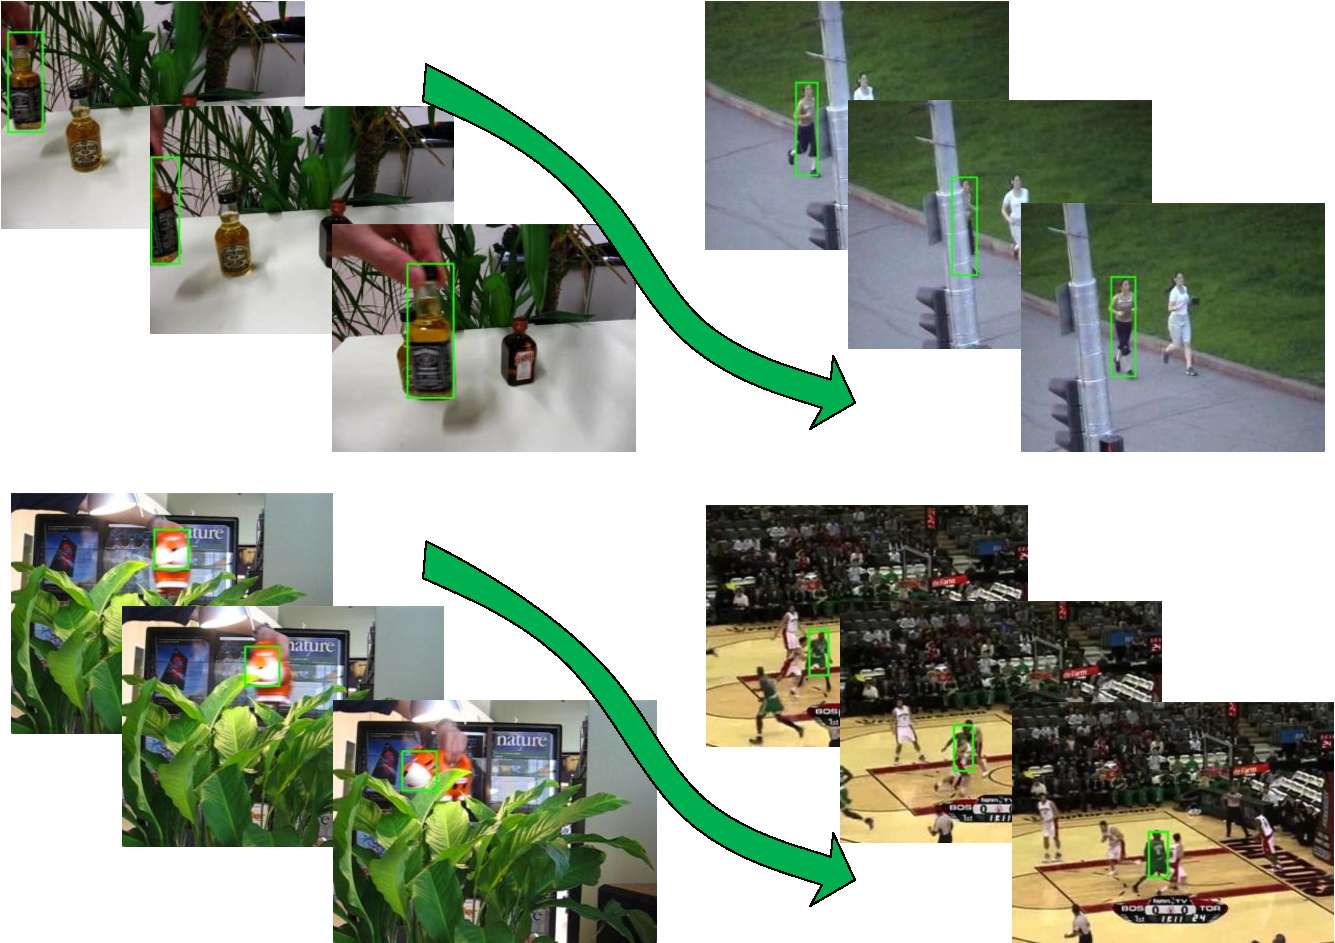
\includegraphics[width=12cm]{intropic1.pdf}
\caption{单目标视觉跟踪示例}
\label{intropic1}
\end{figure}

作为计算机视觉的核心问题之一,视觉跟踪已经被研究了近三十年。
然而随着计算机性能的不断提升、视频采集设备的不断改进、视频数据数量和质量的不断提高、
人们对于智能化的需求不断增加,
视觉跟踪研究不仅从未中断,还引起了研究者们越来越多的关注。
但是,视觉跟踪至今仍然是一个极具挑战性的问题,其面临的困难有\upcite{50seqs}:
\begin{compactitem}
\item 三维空间物体向二维图像投影而产生的信息变化和丢失;
\item 图像采集过程中产生的噪声和畸变;
\item 复杂随机运动、突发运动等难以建模的突发、偶发情况;
\item 物体运动中的非刚性形变;
\item 运动物体被部分或全部遮挡,或者离开可视范围;
\item 光照变化、复杂背景、相似物体、运动模糊、分辨率较低等干扰因素。
\end{compactitem}
除了上述困难外,视觉跟踪系统通常还面临着实时性的挑战。典型地,如果视觉跟踪
的运算时间过长,运算出的结果(即启动运算时的物体位置和状态)对于快速运动中的物体来说已毫无意义。

\begin{figure}[htb]
\centering
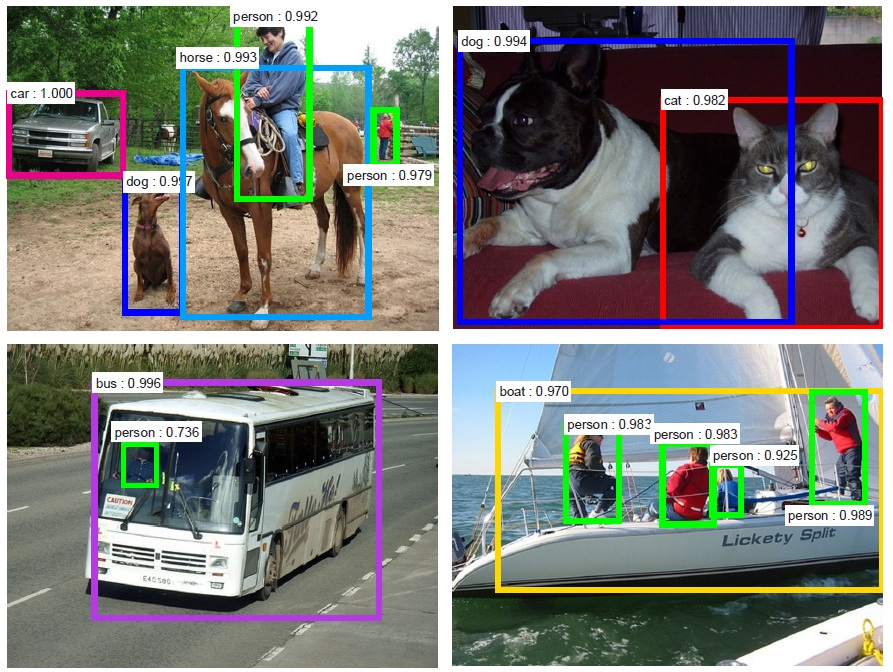
\includegraphics[width=12cm]{introclassification.jpg}
\caption{物体检测示例\upcite{rpn}}
\label{introclassification}
\end{figure}

值得注意的是,当前方兴未艾的物体检测(Objec Detection)技术已经可以给出视野中
物体的种类及其位置,或者定位出属于目标类别的物体,如图\ref{introclassification}所示。
但是,直接将物体检测方法应用
于视觉物体跟踪是不可行的。
首先,计算机视觉的最终模拟对象\pozhehao 人类视觉系统,并不是依靠不
断地检测和分类物体来追踪物体运动的。
即使是从未见过的物体,人类视觉系统仍然能够捕
捉其运动轨迹。
其次,视觉物体跟踪通常有着更高的实时性和精确度要求,而当前常用计算平台的运算能力尚不能满足
物体检测的巨大计算负荷。
如果视觉跟踪的运算时间过长,将无法
被应用于实时跟踪场景;
如果精度不足,``在哪里''的问题也无法解决,严重影响上层应用的功能。
此外,物体的不断运动还会导致非刚性形变、运动模糊、物体旋转、部分离开视野、遮挡、
相似物体干扰等物体检测难以应对的障碍。
但是视觉跟踪则可以根据物体的历史状态以及上下文
环境不断地进行在线学习,从而具有更强的鲁棒性和适应力。
最后,物体检测所面向的并非是某一特定目标,而是一类或者多类物体。
然而视觉跟踪的应用场景往往要求跟踪特定的目标,例
如某一特定车辆或者人物。
区分特定目标和同类相似目标的差别正是视觉跟踪特有的能力之一。

综合上述,视觉跟踪问题是计算机应用领域中一个极其重要、不可替代的基础性理论
问题,长期在学术界倍受关注;同时又有着非常广泛的实际应用,具有极高实用价值;其
本身面临的众多挑战和不断提高的应用需求,确立了其研究价值和前景。
因此,本文选择以视觉跟踪作为研究对象,开展高性能视觉跟踪关键技术研究。


\subsection{高性能视觉跟踪}
本文以``高性能视觉跟踪关键技术研究''为题,其研究意义除了包括上一节所述的,
``视觉跟踪''本身所具有的理论意义和实用价值,
更重要的意义在于``高性能''这一目标。
本文的``高性能''包括了两个方面的内容\pozhehao 
跟踪算法本身的高性能和跟踪算法的高性能实现。

跟踪算法本身的性能由以下4个方面共同构成\upcite{Yang2011}:
\begin{compactitem}
\item 准确性(Accuracy)\pozhehao 跟踪算法所输出的目标物体位置、大小、宽高比等状态信息的准确程度;
\item 鲁棒性(Robustness)\pozhehao 跟踪算法在遮挡、光照变化、相似物体干扰、背景杂乱等跟踪障碍存在的情况下保持准确跟踪的能力;
\item 适应力(Adaptability)\pozhehao 跟踪算法在目标物体本身发生复杂运动、形变、旋转等情况下保持准确跟踪的能力;
\item 效率(Efficiency)\pozhehao 跟踪算法的计算复杂度和运行速度。
\end{compactitem}
通过提升算法本身的上述性能,可以拓展视觉跟踪的应用范围,增强其实用性,
从而从根本上提高计算机视觉上层应用的性能。
此外,研究高性能视觉跟踪算法还需要综合运用信号处理、模式识别、机器学习等多个领域的前沿技术,
有利于多领域的算法理论交叉融合。
同时,跟踪算法的研究成果也将对这些领域的理论研究起到推进作用。

要达到高性能视觉跟踪,还需要探索跟踪算法的高性能实现。
这里的高性能实现,和``高性能计算''属同一范畴,意指在算法的编程实现过程中,
针对底层硬件体系结构特征,
充分发挥计算设备/平台的计算能力,
提高所实现的算法的运行效率。
提高跟踪算法实现的性能将起到以下重要作用:
\begin{compactitem}
\item	提高算法的运行效率,使得计算复杂度较高的算法仍然可以达到实时跟踪的要求;
\item	使得跟踪算法能够适用于更加复杂的跟踪场景、更高的图像分辨率、以及对实时性要求更高的场合;
\item	使得同时启用多个算法实例来同时跟踪多个目标变得可行;
\item	大部分跟踪算法需要在运行效率和跟踪精度间进行折衷,而算法的高性能实现可以提高对计算复杂度的容忍度,从而提升跟踪精度。
\end{compactitem}

借助于向量运算单元、流水线、多核并行等体系结构技术,
通用处理器(CPU)的计算能力得以保持较高速度的增长。
但是简单直接的算法实现并不能充分发挥CPU的性能,
如何开发跟踪算法的并行性以及如何利用高速缓存(Cache)、向量单元等体系结构要素,
是在CPU上进行算法高性能实现的关键。
以GPGPU为代表的众核加速器与通用处理器相比,在性能和功耗上都有着较大的优势。
但是在其上进行算法实现时,需要将计算负载映射至众核设备上运行,即需要对传统的串行程序进行体系结构特定的并行化改造。
由于算法/程序本身特征的限制,这种并行化所能达到的程度有所不同;
编写优质高效的并行程序,还需要对众核设备的体系结构和编译机制有着深刻的理解,
这对算法实现者有着很高的要求。
上述两点往往限制了众核加速器的利用效率,使得算法实现的实测性能和设备峰值性能间的差距巨大。
从嵌入式系统到大规模计算集群,上述通用处理器和众核加速器杂合的异构计算平台正被广泛使用。
如何同时发挥通用处理器和加速器的性能,以及如何控制两者间的协作和数据传输等,是高性能算法实现面临的又一挑战。
当前,视觉跟踪这一重要算法在异构计算平台下的高性能实现还缺乏足够的研究工作,
开展该项研究可以填补空白,具有极高的实用价值;
同时,该项研究还可以对并行程序设计、并行编译和体系结构等领域的研究起到牵引作用;
此外,研究跟踪算法的高性能实现还需要对算法进行深入理解和改造适配,如进行并行化、模块间解耦合等,
从而推进跟踪算法本身的研究和进步。


\section{研究现状}

\subsection{经典视觉跟踪算法的研究现状}
通过总结视觉跟踪算法的普遍结构,以及参考综述文献\cite{50seqs, Yang2011, Smeulders2014, Wang2015}中对于视觉跟踪器结构的分析,
本文认为一个完整的经典视觉跟踪算法通常具有如图\ref{introtrackerstruct}所示的结构:

\begin{figure}[htb]
\centering
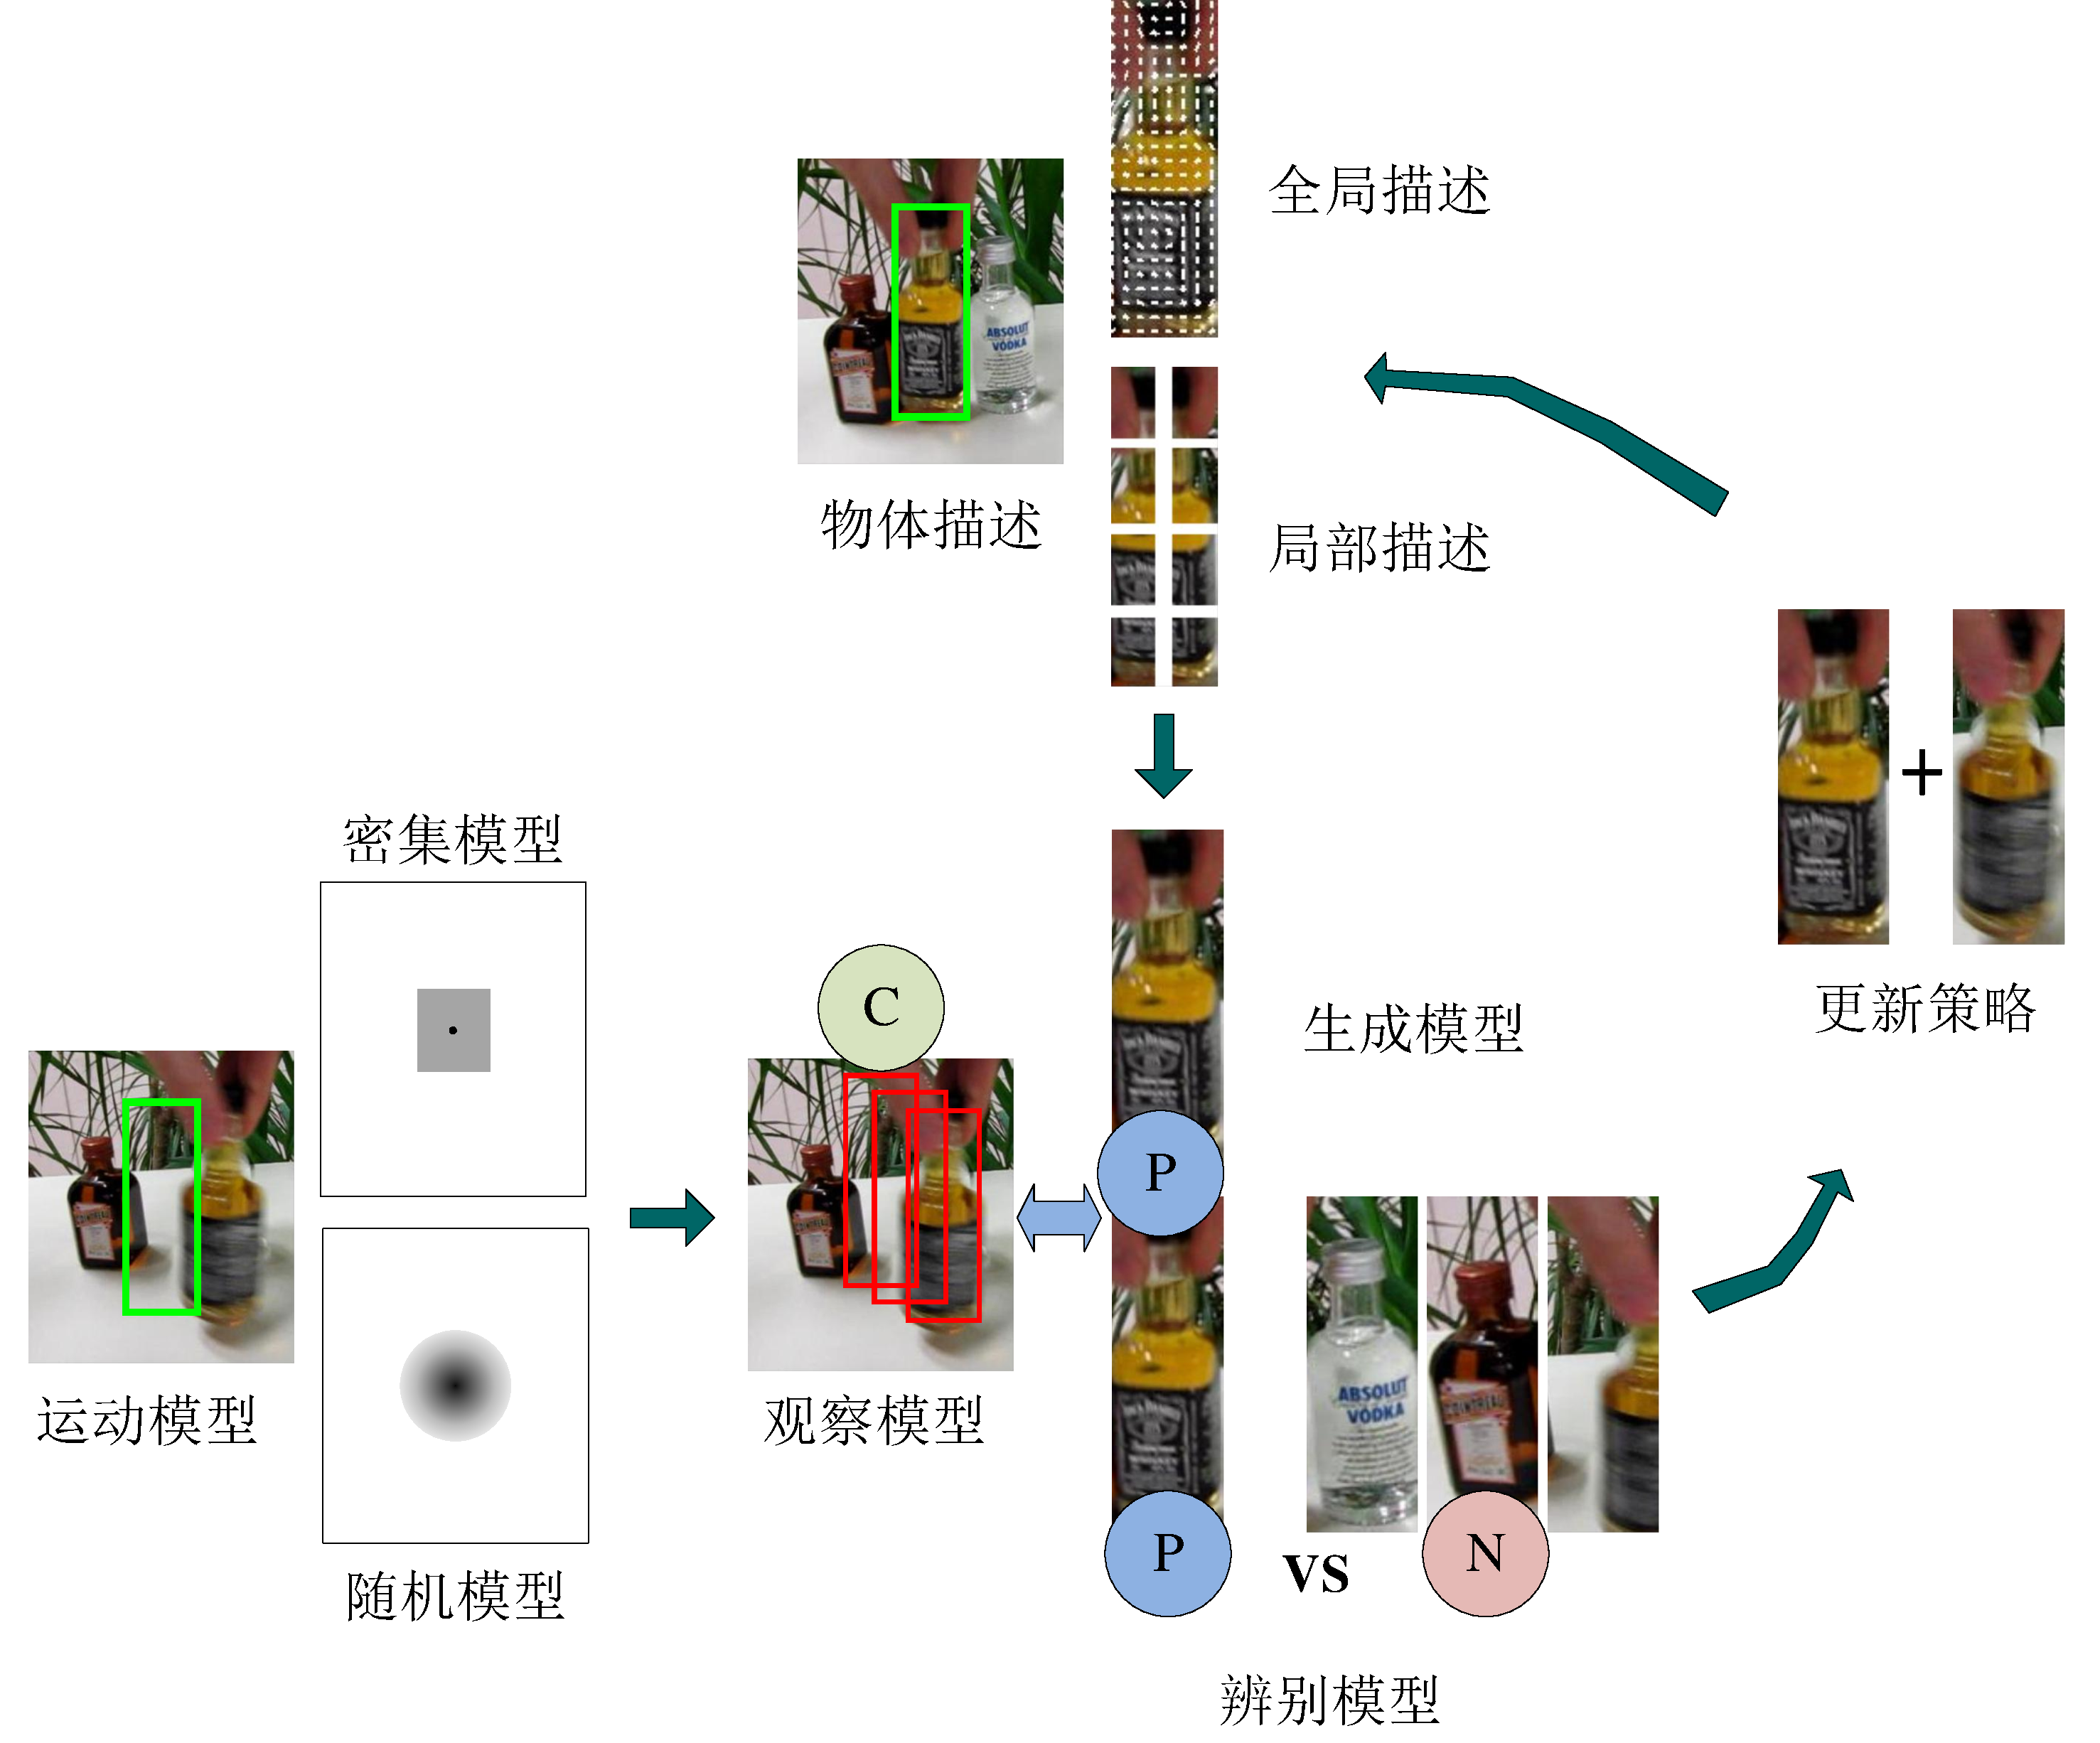
\includegraphics[width=12cm]{introtrackerstruct.pdf}
\caption{经典视觉跟踪算法的结构}
\label{introtrackerstruct}
\end{figure}

\begin{compactitem}
\item	\textbf{物体描述(Object Description)}:用于建模目标物体的外观特征,使得目标物体得以与其它物体或者背景区分开来。当前主要有两种类型\pozhehao 全局描述\upcite{act, kcf, vtd}和局部描述\upcite{asla, lsk, scm}。前者通常是一个整体的结构性特征块(Structured Feature Patch),后者通常将物体分为多个特征子块,这些子块形成一个特征“字典(Dictionary)”。
\item	\textbf{运动模型(Motion Model)}:用于根据目标物体的历史运动轨迹和前序状态来提取候选区域(图\ref{introtrackerstruct}中用``C''表示),这些候选区域将被用于进一步的判断。运动模型通常可分为两大类:密集模型(Dense Model)\upcite{kcf, csk, dsst, samf}会穷举所有可能的候选区域;而随机模型(Random Model)\upcite{vtd, asla, scm}将根据某种概率分布,随机地采样候选区域。
\item	\textbf{观察模型(Observation Model)}:用于根据物体描述,判断候选区域内存在目标物体的可能性,从而找出最为准确的当前目标位置和状态。两大类观察模型中,辨别模型(Discriminative Model)\upcite{kcf, csk}能够显式地建模正样本(图\ref{introtrackerstruct}中用``P''表示)和负样本(图\ref{introtrackerstruct}中用``N''表示)的区别;而生成模型(Generative Model)\upcite{vtd, asla, lsk}仅建模候选区域内的图像块和物体描述的相似性。
\item	\textbf{更新策略(Updating Scheme)}:用于在跟踪过程中不断更新物体描述和观察模型。由于目标物体的外观在运动过程中会不断改变,更新策略是提高跟踪器鲁棒性和适应力的必备模块。
\end{compactitem}

总结经典跟踪算法的发展,可以发现其各个模块都在不断进步。
物体描述方面,早期跟踪器通常直接采用灰度值或颜色值。
而当前的跟踪算法中,颜色名(Color Naming)\upcite{act, colornaming, samf}、
颜色直方图(Color Histogram)\upcite{colorhistogram}、灰度直方图(HoG)\upcite{kcf, dsst, samf, hog}、
霍尔梯度(Haar Gradients)\upcite{struck}等各种各样的特征描述均被采用,
甚至出现了整合多种特征的趋势\upcite{act, samf, kcfdp}。
相对于直观简单的全局描述\upcite{mosse, struck},将目标外观分解为多个部分看待的局部描述\upcite{asla, lsk, scm}可以更好地处理物体形变和遮挡等问题,
目前已被广泛采用。
观察模型中,生成模型\upcite{vtd, asla, lsk}较为简单直观,仅能建模从当前物体描述来生成当前目标外观的可能性;
而新出现的辨别模型\upcite{kcf, csk, tld, tldjournal}通常训练一个分类器,
不仅考虑候选区域中的图像块与正样本的相似性,还考虑它与负样本的区分度,
从而更鲁棒地辨别目标区域和非目标区域。
运动模型比较多样。
在早期的跟踪算法中,隐式运动模型\upcite{lsk}将对目标位置的预测隐藏在一个最优化过程中。
而基于高斯运动模型的采样方法一直在被广泛采用,如点滤波(Particle Filtering)\upcite{asla, scm, multicue}。
均匀采样或者密集采样方法会在目标的历史位置附近进行密集且均匀地搜索,是最为鲁棒也是最为耗时的方法。
此外,还有结合多个高斯模型的马尔科夫蒙特卡洛(Markov Chain Monte Carlo)方法\upcite{vtd},
以及可以进行运动预测的卡尔曼滤波(Kalman Filter)方法\upcite{kalman}等。
将运动模型和全视野内物体检测相结合的方法目前也在兴起\upcite{tld, tldjournal}。
早期的跟踪算法通常不进行模型更新,而近年来的跟踪器都会采用适合自身物体描述和观察模型的更新策略。
从最简单的线性插值\upcite{kcf, csk, samf}到最复杂的步步为营(Boot-Strapping)法在线重训练\upcite{tld, decitree},
各种更新策略层出不穷。

\subsection{结合物体检测技术的新兴视觉跟踪算法研究现状}
在最近几年中,随着互联网大数据的爆发式增长,
以及深度学习、卷积神经网络(Convolutional Neural Network,CNN)等基础理论的巨大成功,
物体分类和物体检测成为了炙手可热的研究领域。
在视觉跟踪方面,最新的跟踪算法也通过引入物体检测领域的方法,
使得精度、鲁棒性和适应力获得了很大提升。
当前,在跟踪算法中融合物体检测技术已经成为一种趋势,继而诞生出一批新兴的视觉跟踪算法。

最早加入物体检测模块的跟踪器是TLD\upcite{tld, tldjournal},
它将跟踪器重新解耦合为三大模块:跟踪(Tracking)、学习(Learning)和检测(Detection)。
跟踪模块通过Lucas-Kanade方法\upcite{lkoptflow}计算稀疏光流,并在两帧间估计连续、简单的物体运动;
检测模块在整幅图像(跟踪器视野范围)内通过Fern随机森林和最邻近分类器来检测可能包含目标的区域;
学习模块负责把检测模块和跟踪模块的输出进行对比整合,同时还按照P-N学习的策略,
根据物体的运行轨迹提取正、负样本,并更新其分类器。

使用物体检测领域中强大的分类器(如CNN)来作为跟踪算法的物体描述和观察模型也是当前的一大潮流。
在2015年的视觉跟踪竞赛VOT 2015\upcite{vot2015}上,MDNet\upcite{mdnet}取得了第一名。
它建立了一个专门面向视觉物体跟踪的6层CNN。
该网络具有提取目标外观特征(物体描述)和评价候选区域(观察模型)两方面的作用。
在每一帧中,MDNet首先按照高斯分布对目标物体的位置和尺度大小进行采样(运动模型),
采样结果将被独立地输入CNN进行评价。
MDNet的模型更新策略就是利用新的目标状态来对CNN再次进行微调训练(Fine-Tunning)\upcite{rcnn}。
通过利用当前物体检测领域最为有力的卷积神经网络,MDNet取得了当前最高的跟踪精度和鲁棒性。
但是,较为复杂的网络结构、大量的采样样本导致了极低的跟踪效率(在高性能GPU服务器上达到1 FPS)。
类似MDNet的方法还有DLT\upcite{deepimage}(使用堆叠去噪自动编码器网络),
SO-DLT\upcite{sodlt}(使用2个具有7层卷积层的深度CNN),
以及DeepTrack\upcite{deeptrack}(使20个CNN组成的CNN池以处理不同特征)等。

DeepSRDCF\upcite{deepsrdcf}在VOT 2015中取得了仅次于MDNet的成绩,
但其理念略有不同:它首先在ImageNet数据集\upcite{imagenet}上预训练一个用于物体分类的5层CNN网络,
然后利用该网络的第1层卷积层来提取特征作为物体描述,
并使用了对偶相关滤波(DCF)\upcite{kcf}来作为观察模型对提取的特征进行辨别。
DeepSRDCF证明,深度神经网络自动学习到的特征大大优于人为设计的特征描述,
可以获得极高的跟踪精度和鲁棒性,
但是较大的计算负载却使得运行效率难以保证。

上述跟踪器效率较低的另一原因是大量地采样候选区域并且对候选位置进行逐一地评价。
为了解决这一问题,目标候选(Detection Proposal)这一物体检测领域的新兴方法也被引入跟踪器中,
对提高适应力、鲁棒性和跟踪效率均有着突出的贡献。
目标候选方法能够十分高效地在一幅图像中提取出可能包含物体的区域,
这些区域将作为分类器的输入,
从而避免了在图像中进行密集的搜索和采样。
EdgeBoxes\upcite{edgeboxes}是当前最为成功的目标候选生成方法之一,
它假设一个矩形区域中所包含的完整物体边界数量与其包含物体的可能性是正相关的。
大量实验和实际应用也证明了这一假设是可行的。
基于EdgeBoxes,EBT\upcite{ebt}直接从整幅图像中提取目标候选区域,
以应对物体的随机、快速运动。
它还通过训练一个线性SVM来对EdgeBoxes的输出区域进行重新排序,大幅减少了需要进一步辨别的候选区域。
%KCFDP\upcite{kcfdp}和KCFDPT\upcite{kcfdpt}也基于EdgeBoxes,但它们将目标候选生成器作为密集采样运动模型的一个补充,
%以提高跟踪算法的适应力和鲁棒性。

\subsection{高性能视觉跟踪算法实现的研究现状}
要达到``高性能视觉跟踪''这一目标,除了算法层次的优化改进以外,
充分利用计算平台的计算资源,进行高效的算法实现也是同等重要的。
当前,包含两类甚至多类计算设备的异构计算平台是从嵌入式计算领域到超级计算应用的普遍选择,
也是各种高性能算法实现的首选硬件平台。
因此,本文高性能视觉跟踪算法的实现也将重点关注异构计算平台。
目前,异构平台上的高性能视觉跟踪算法实现还比较少,但是仍然有着一些代表性的工作。

在早期的跟踪器中,由于缺乏像深度神经网络那样的重负载、高精度的观察模型,
因此通常着重于运动模型的高性能实现。
点滤波(Particle Filtering)是早期跟踪器中最为常用的运动模型,
它对于运动较为规律、较少突发、随机运动的物体具有较好的跟踪效果。
点滤波跟踪器通常在初始化过程中均匀地采样大量样本点,然后通过这些样本点估计出物体可能的运动模型(一个概率密度函数)。
在新的图像帧到来时,它在物体最可能出现的位置附近多采样,而在可能性较低的位置少采样,
从而在跟踪精度和运行效率方面进行折衷。
在得到目标物体的新位置后,通常还需要更新上述概率密度函数,以提高运动模型的适应力。
点滤波过程中采样点的数目通常成百上千。
为了提高准确性和适应力,每个点数据通常还要加入宽度、高度甚至旋转角度等信息,导致点数据的维度较高。
因此迫切需要对点滤波跟踪算法进行高性能的实现。
\cite{Concha2014}将点滤波器分解为几个步骤:初始化、评权、判断、选择和扩散,
并且将每一个步骤分别在CPU和GPU上进行了高性能的实现和评测。
该实现和评测显示,在采样点数量较大时,GPU相比CPU具有更大的优势。
最后,他们还给出了一个在异构平台(CPU+GPU)上实现的完整跟踪器结构,
即CPU负责采集图像、初始化和判断步骤,而GPU通过3个Kernel程序实现其余步骤。
其中选择和扩散步骤被证明适于融合在一个Kernel中。
\cite{Brown2012}提出了一个用于三维物体跟踪的高性能点滤波跟踪器框架,
并在刚体跟踪和手势跟踪上取得了成功。
该框架的核心是点滤波器在GPU上的精细实现和优化,
以充分开发采样点间的并行性和像素级的并行性。
主要的计算负载在GPU上被分为3个Kernel,即图像分割和特征提取(像素级并行)、像素和像素块权值计算(像素级和采样点间并行)、
以及采样点权值计算(采样点间并行)。
此外,精细的存储空间划分和面向GPU存储层次的适配也是该框架性能优异的关键。
\cite{Rymut2010}中使用了“点涌动(Particle Swarm)”方法,它是点滤波的一个变型,
即用每个采样点的移动代替了重新采样,并且各个点的移动会互相影响而不是像点滤波中那样的完全独立。
由于算法上复杂度的降低,2个Kernel程序被分别用于计算归一化方差和计算采样点与模板的匹配度。
最后,目标物体的当前位置将通过并行归约计算得到。
其它在GPU上实现的高性能点滤波跟踪算法还有\cite{Cabido2012}(除目标位移外还考虑了尺度变化和旋转角度)
和\cite{Lozano2009}(专门面向人脸跟踪)。

TLD跟踪器的高性能实现也获得了一定关注。
如上一节所述,TLD将跟踪器分解为松耦合的三大模块,即跟踪、学习和检测。
这使得除了Kernel内的并行优化以外,过程间并行和延迟隐藏等高性能实现技术也成为可用的优化手段。
\cite{htld}在CPU+GPU异构平台上,使用OpenMP\upcite{openmp}和CUDA\upcite{cudaspec}实现了TLD的高性能版本\pozhehao H-TLD。
它除了充分利用CPU上的多核和GPU的数据并行单元以外,
还通过合理的CPU、GPU负载分配和数据流压缩技术有效地降低了数据传输开销。
此外,检测模块和数据传输的重叠执行(利用异步复制引擎)也起到了延迟隐藏的作用。
\cite{Pengyu2013}是CPU+GPU异构平台上的另一个高性能TLD实现版本,
它首先在算法上对TLD进行了改进,包括在线生成检测模块的尺度空间、使用点滤波代替检测模块的全图搜索等。
然后通过将跟踪模块和检测模块重叠执行,提高了跟踪效率。


\subsection{异构平台下高性能编程模型的研究现状}
异构计算平台的广泛应用和不断发展,让高性能的算法实现面临着更多的挑战。
异构计算平台上CPU 和GPU(或者其它加速器)体系结构的差别,导致了各自完全不同的编程优化方法。
开发者通常要为不同的计算设备进行不同版本的优化实现,或者退回到比较保守的通用实现,
但这会带来较大的性能损失。
因此,难以编程,以及缺少统一的编程框架或者编程模型,是异构计算平台面临的最大问题之一。

研究表明,适用于各种异构计算设备/平台的普适性编程模型几乎不存在\upcite{Hill2012}。
例如,共享存储的多处理器(Shared Memory Multiprocessors)通常使用OpenMP或Pthread一类的线程级并行语言;
而GPU类的众核加速器通常使用数据级并行模型(如StreamC/KernelC\upcite{streamc},CUDA);
多机、多节点间的通讯通常采用消息传递类编程模型,如MPI\upcite{mpi},以及这个层次的MapReduce,Dryad\upcite{dryad},P2G\upcite{Espeland2011}等。
太多的编程模型增加了编程者的负担,并且有些编程模型之间甚至是互斥的。

在当前的异构平台上,可用于视觉跟踪算法高性能实现的编程模型包括三类,即开发数据级并行的编程模型,程序员控制调度的编程模型,以及领域专用语言。

第一类编程模型需要程序员显式地管理并行任务划分、同步、存储分配等,因此面向体系结构的优化是无法避免的,
代码通常需要为不同计算设备进行重新改写。
例如流语言StreamC/KernelC,它虽然是典型的用于媒体计算的编程框架,
但却是专门面向Imagine\upcite{streamc}流体系结构设计的,不能适应多核处理器以及新兴的GPGPU。
CUDA\upcite{cudaspec}编程模型的情况尤甚,仅能用于Nvidia的GPU产品。
但是OpenCL\upcite{oclspec}是个例外。它是跨架构的统一编程模型,被众多计算设备所支持,
例如多核CPU、各厂商的GPU、Cell处理器\upcite{cell}、Xeon Phi加速器\upcite{mic}等。
虽然OpenCL程序可以不加修改地运行在不同设备/平台上,即具有很好的功能移植性,
但是其性能可移植性并不令人满意,这一点在体系结构差别较大的情况下尤为突出。
例如,为GPU加速器编写的OpenCL程序不可能同样高效地运行在多核CPU上,
必须进行面向体系结构的改写\upcite{Lan2012}。
这一问题的根本原因在于,OpenCL抽象所有的目标平台为统一的平台模型、存储模型和执行模型,
但在真实环境中目标平台是多种多样的,程序员需要为不同的平台制订平台特定的优化策略\upcite{Seo2011}。

第二类编程模型,如Sequioa\upcite{Fatahalian2006},需要用户定义一种映射模型来描述如何将计算任务运行在一个树状的存储层次上。
但是它面向的是抽象的存储层次,因此仍然需要程序员去了解具体硬件细节,并进行手动地适配。
此外,Sequioa的关注重点在于任务调度,在细粒度的并行方面并没有太大优势。

第三类编程模型的典型例子是Matlab。
虽然领域专用语言的高级语法使得程序变得非常简洁,并且配备有大量的库函数支持,
但是它仅针对基本计算负载(如矩阵乘法等)进行了优化,且使用了低效的解释执行机制。
因此对于整个算法来讲,Matlab程序通常较为低效。

其它的编程模型也暴露出不少的缺点,例如Map-Reduce的问题包括\upcite{Catanzaro2010}:
1)启动开销大,即使是简单任务也要经历Map-Shuffle-Reduce三个过程,无法做到快速响应;
2)只能处理静态数据,对变化较快的数据(如实时跟踪时不断采集的图像)无能为力;
3)MapReduce的具体实现至今仍是Google的机密,现有的开源版本效率低下。

国际学术界也为编程模型做了许多有价值的研究\upcite{Catanzaro2010}。
Berkeley的学者期望应用领域专家使用快速编程语言,例如Python等,来编写算法;
而编程效率专家则使用C语言等来为快速编程语言编写高效库函数。
Stanford的学者的观点相对激进,他们基于Scala语言开发出一个计算框架Delite\upcite{Lee2011}。
编程效率专家可以使用Delite来开发领域专用的语言(Domain-Specific Language,DSL),以供领域专家使用。
Delite框架把基于DSL语言开发的程序转换成一种中间表示, 并进行面向领域的并行优化,
从而产生适于不同计算设备的可执行代码。
MIT、Stanford和Adobe的学者针对图像处理提出了一种新的DSL语言\pozhehao Halide\upcite{Kelley2012}。
Halide提供了可面向具体硬件进行配置的调度器,
还基于LLVM\upcite{llvm}改造了一个编译环境,
以产生面向不同体系结构的可执行代码。
韩国学者在OpenCL编程模型下,
尝试了将单节点上的多GPU虚拟成一个GPU,以及将集群中的多节点虚拟成单节点\upcite{Kim2011}。


\section{主要研究内容和创新点}
综合考虑当前高性能视觉跟踪算法和跟踪算法高性能实现的研究现状,本文认为,
要达到高性能视觉跟踪,还存在着一些问题。
首先是经典视觉跟踪算法的鲁棒性和适应力普遍不足,难以有效跟踪形变较大、变化较快的物体。
其次,在结合物体检测技术的跟踪算法中,由于大量随机采样所造成的较低运行效率是一个突出问题。
此外,现有的高性能跟踪算法实现通常面向某一特定的硬件计算设备/平台,难以向不同的计算设备/平台进行移植。
使用OpenCL进行跟踪算法的高性能实现可以保证功能上的良好移植性,
但是由于其性能移植性上的问题,
导致面向特定体系结构优化后的OpenCL程序,难以在不同体系结构的计算设备上取得同样的性能提升。

因此,本文的主要研究内容有以下几点:

\begin{compactitem}
\item[1.]
针对视觉跟踪算法对目标物体的尺度和宽高比变化适应力不足这一问题,
本文将物体检测领域最有潜力的``目标候选''生成方法之一\pozhehao EdgeBoxes,
和当前最为高效的跟踪算法之一\pozhehao 基于相关滤波的跟踪算法,进行了紧密结合。
为了能够准确辨别大小、形状多变的目标候选,本文对相关滤波跟踪算法的物体特征描述和更新策略进行了优化;
为了提高嵌入目标候选后的跟踪效率和鲁棒性,本文在跟踪过程中加入了目标候选过滤和带阻尼的更新步骤。
两者结合所得的跟踪器在一个大型公开测试集上展现出了很强的鲁棒性和适应力,
同时还达到了令人满意的跟踪速度。

\item[2.]
为了深入分析跟踪算法中``目标候选''的作用,本文将多种具有代表性的目标候选生成方法分别
面向跟踪任务进行了适配,并和优化后的相关滤波跟踪算法相结合。
通过对比分析这些目标候选生成方法在跟踪过程中的表现,本文证明了目标候选在视觉跟踪中有着重要作用,
且其质量和跟踪精度间存在着正相关的关系。
此外,本文还针对跟踪算法的特点,在EdgeBoxes中加入了``背景抑制''这一优化步骤,
有效弥补了EdgeBoxes容易受到非目标物体边界干扰这一缺陷,
使得物体检测领域的目标候选方法更加适用于视觉跟踪。

\item[3.]	
为了研究异构计算平台上可移植的视觉跟踪算法高性能实现,
本文基于通用并行编程模型OpenCL,对TLD跟踪算法进行了高性能的并行实现。
通过分析和提取TLD算法的计算密集部分和瓶颈部分,本文并行化了Fern随机森林的特征提取和分类过程、
最邻近分类的NCC计算过程、以及学习过程中的重叠率计算和正负样本提取。
此外,由于Fern随机森林和LK光流跟踪互相独立,本文还在不同的计算设备上将它们重叠执行。
由于性能移植性问题的存在,各个Kernel程序将运行在各自适合的计算设备上,最终取得了令人满意的整体加速比,
完全满足实时跟踪的需求。

\item[4.]	
为了解决使用OpenCL进行视觉跟踪算法高性能实现所面临的性能移植性问题,
本文提出了一套新的代码转换方法,该方法能够有效地提升GPU特定的Kernel程序在多核/众核CPU上的性能移植性。
借助于本文新提出的数组访问描述式,在工作项折叠过程中,
所有的冗余局部存储数组和对应的同步都将被消除。
在Kernel的后继优化过程中,本文不仅从原GPU特定Kernel中提取并行性和局部性信息,
还会考虑目标CPU的体系结构细节,以进一步提升Kernel程序在CPU上的性能。
实验表明,GPU特定的Kernel程序在使用本文的代码转换方法后,将在CPU上获得明显的性能提升。
借助这一研究成果,在异构平台上实现高性能跟踪器时,可专注于面向GPU的优化,或是重用已有的GPU特定代码。
\end{compactitem}

在以上研究内容中,本文的突出贡献和主要的创新点有:
\begin{compactitem}
\item[1.]
在作者所知范围内,本文是最早将物体检测领域常用的``目标候选''方法应用于视觉物体跟踪中的。
通过本文的优化和整合,目标候选的高度灵活性和相关滤波器的准确辨别力将互相补充,
大幅提升视觉跟踪算法的适应力和鲁棒性,并同时保证足够的跟踪效率。
此外,本文提出的方法还是一个通用方法,可用于将不同的目标候选生成方法和不同的跟踪算法相结合。

\item[2.]
通过将多个不同的``目标候选''生成方法面向跟踪任务进行适配,并融入跟踪算法中,
本文首次证明了目标候选对于视觉跟踪的重要作用,并揭示了候选质量和跟踪精度间的正相关关系。
基于上述发现,本文还针对跟踪需求优化了目标候选生成方法,明显提升了目标候选对于视觉跟踪的适用性。

\item[3.]	
在异构计算平台上,本文首次基于可移植的并行编程模型OpenCL,对TLD这一完整跟踪应用进行了高性能并行化。
通过对TLD算法进行分析和分解,本文将其计算密集和性能瓶颈的部分进行了高性能实现,
并指定对应的Kernel程序运行在各自适合的计算设备上,从而取得了令人满意的跟踪性能。

\item[4.]	
针对GPU特定的OpenCL Kernel程序在CPU上的性能移植性不佳这一问题,
本文提出了一种新的代码转换方法。
该方法解决了现有方法普遍忽略的两个重要问题:一是使用局部存储数组可能对CPU上的性能带来负面影响;
二是忽略或者盲目继承GPU特定Kernel中的数据局部性可能带来性能损失。
实验表明,对于GPU特定的Kernel程序,若使用包含本文方法的新OpenCL运行时,
将取得超越Intel官方运行时的性能。
\end{compactitem}

\section{论文结构}
本文共分为六章,具体结构如下:

第一章为绪论,介绍本文进行高性能视觉跟踪关键技术研究的背景和目的,总结当前视觉跟踪研究的现状,
并针对现状提出本文的两大研究要点\pozhehao 视觉跟踪的高性能算法和跟踪算法的高性能实现。

第二章介绍一种将物体检测领域常用的``目标候选''方法用于视觉跟踪的通用方法。基于该方法,
本文将目标候选生成器EdgeBoxes和基于相关滤波的跟踪器KCF相结合,大幅提高了视觉跟踪对于物体尺度和宽高比变化的适应力。

第三章介绍如何将多个不同的目标候选生成器面向跟踪任务进行适配并嵌入跟踪器中,
以及如何对EdgeBoxes进行针对视觉跟踪的改造优化。
实验和评测揭示了目标候选在视觉跟踪中的作用,同时也证明了对EdgeBoxes的优化是十分有效的。

第四章在CPU+GPU的异构计算平台上,以OpenCL作为编程模型,
对完整的TLD跟踪算法进行了高性能的实现。
通过并行化TLD的计算密集部分和性能瓶颈部分,以及在多设备上进行重叠执行,本文展示了视觉跟踪算法在异构平台下的
高性能实现所需的关键技术和面临的问题挑战。

第五章针对OpenCL所暴露出来的性能移植性问题,提出一套新的代码转换方法。
该方法基于对数组访问的准确线性描述,包含基于分析的工作项折叠和面向体系结构的后续优化等步骤,
能够有效地提升GPU特定Kernel程序在多核/众核CPU上的性能移植性。

第六章对全文进行总结,并介绍未来的进一步研究计划。





